\documentclass[aspectratio=169,12pt]{beamer}
\usepackage[utf8]{inputenc}
\usepackage{amsmath,amssymb}
\usepackage{graphicx}
\usepackage{tikz}
\usetikzlibrary{shapes.geometric, arrows.meta}
\usepackage{hyperref}
\usepackage{listings}
\usepackage{xcolor}

% 主题设置
\usetheme{Madrid}
\usecolortheme{default}
\usefonttheme{professionalfonts}

% 代码高亮设置
\lstset{
    language=Python,
    basicstyle=\ttfamily\small,
    keywordstyle=\color{blue},
    commentstyle=\color{gray},
    stringstyle=\color{orange},
    showstringspaces=false,
    breaklines=true,
    frame=single,
    backgroundcolor=\color{gray!10}
}

% 标题信息
\title{CausalEngine: Making Machine Learning Smarter}
\subtitle{从相关性到因果性的革命 (From Correlation to Causation)}
\author{龚鹤阳 (Heyang Gong)}
\date{\today}

\begin{document}

% 标题页
\begin{frame}
\titlepage
\end{frame}

% 目录
\begin{frame}{今天我们要讲什么? (What are we talking about today?)}
\tableofcontents
\end{frame}

% 第一部分:问题是什么?
\section{传统机器学习有什么问题? (Problems with Traditional ML)}

\begin{frame}{传统机器学习的局限性 (Limitations of Traditional ML)}
\begin{columns}
\column{0.5\textwidth}
\textbf{传统机器学习做什么? (What does traditional ML do?)}
\begin{itemize}
    \item 学习数据中的相关性 (Learn correlations in data)
    \item 就像: 看到乌云就说要下雨 (Like: see clouds, predict rain)
    \item 但不知道为什么下雨 (But don't know WHY it rains)
\end{itemize}

\vspace{1em}
\textbf{问题出现了: (Problems arise:)}
\begin{itemize}
    \item 数据有噪音就不准了 (Fails with noisy data)
    \item 每个人的差异被当作"干扰" (Individual differences = "noise")
    \item 只能告诉你"是什么", 不知道"为什么" (Tells WHAT, not WHY)
\end{itemize}

\column{0.5\textwidth}
\begin{center}
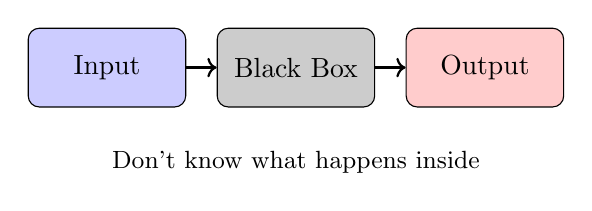
\begin{tikzpicture}[scale=0.8]
% 传统ML示意图
\node[draw, fill=blue!20, rounded corners, minimum width=2cm, minimum height=1cm] (x) at (0,0) {Input};
\node[draw, fill=black!20, rounded corners, minimum width=2cm, minimum height=1cm] (box) at (3,0) {Black Box};
\node[draw, fill=red!20, rounded corners, minimum width=2cm, minimum height=1cm] (y) at (6,0) {Output};
\draw[->, thick] (x) -- (box);
\draw[->, thick] (box) -- (y);
\node at (3,-1.5) {\small Don't know what happens inside};
\end{tikzpicture}
\end{center}
\end{columns}

\vspace{1em}
\begin{alertblock}{核心问题 (Core Problem)}
现实世界的数据总是有噪音的, 传统方法应付不了! (Real-world data is always noisy, traditional methods can't handle it!)
\end{alertblock}
\end{frame}

\begin{frame}{我们需要什么样的解决方案? (What kind of solution do we need?)}
\begin{center}
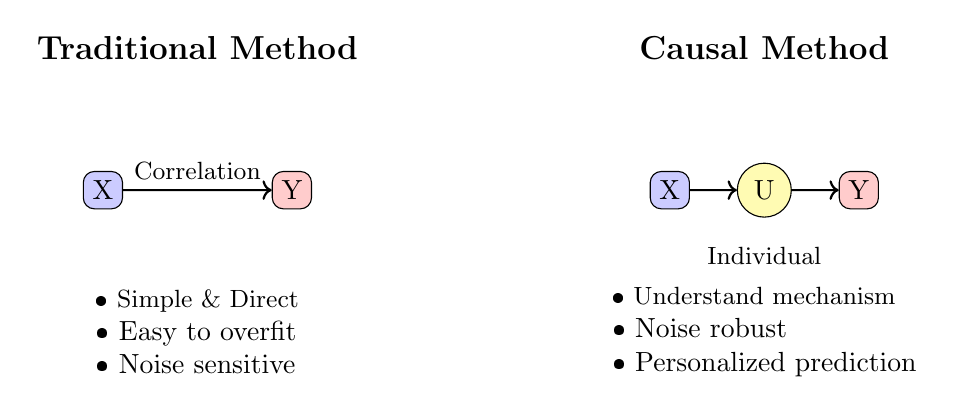
\begin{tikzpicture}[scale=1.2]
% 对比图
\node at (0,3) {\textbf{\large Traditional Method}};
\node at (6,3) {\textbf{\large Causal Method}};

% 传统方法
\node[draw, fill=blue!20, rounded corners] (x1) at (-1,1.5) {X};
\node[draw, fill=red!20, rounded corners] (y1) at (1,1.5) {Y};
\draw[->, thick] (x1) -- (y1) node[midway, above] {\small Correlation};

% 因果方法
\node[draw, fill=blue!20, rounded corners] (x2) at (5,1.5) {X};
\node[draw, circle, fill=yellow!30] (u) at (6,1.5) {U};
\node[draw, fill=red!20, rounded corners] (y2) at (7,1.5) {Y};
\draw[->, thick] (x2) -- (u);
\draw[->, thick] (u) -- (y2);
\node at (6,0.8) {\small Individual};

% 优势对比
\node[align=left] at (0,0) {\small • Simple \& Direct\\• Easy to overfit\\• Noise sensitive};
\node[align=left] at (6,0) {\small • Understand mechanism\\• Noise robust\\• Personalized prediction};
\end{tikzpicture}
\end{center}

\begin{block}{关键洞察 (Key Insight)}
每个个体都有独特的特征U, 这不是噪音, 而是有用的信息! (Each individual has unique feature U - this is not noise, but useful information!)
\end{block}
\end{frame}

% 第二部分:因果引擎怎么工作?
\section{因果引擎是怎么工作的? (How does CausalEngine work?)}

\begin{frame}{因果引擎的四个步骤 (CausalEngine's Four Steps)}
\begin{center}
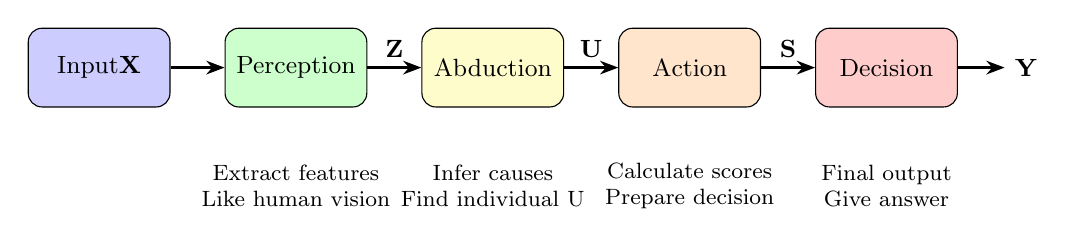
\begin{tikzpicture}[
    scale=1,
    box/.style={draw, rounded corners=5pt, minimum width=1.8cm, minimum height=1cm, font=\small},
    arrow/.style={->, thick, >=Stealth}
]

% 主要流程
\node[box, fill=blue!20] (X) at (0,0) {Input\\$\mathbf{X}$};
\node[box, fill=green!20] (P) at (2.5,0) {Perception};
\node[box, fill=yellow!20] (Ab) at (5,0) {Abduction};
\node[box, fill=orange!20] (Ac) at (7.5,0) {Action};
\node[box, fill=red!20] (D) at (10,0) {Decision};

% 箭头和中间变量
\draw[arrow] (X) -- (P);
\draw[arrow] (P) -- (Ab) node[midway, above, font=\small] {$\mathbf{Z}$};
\draw[arrow] (Ab) -- (Ac) node[midway, above, font=\small] {$\mathbf{U}$};
\draw[arrow] (Ac) -- (D) node[midway, above, font=\small] {$\mathbf{S}$};
\draw[arrow] (D) -- ++(1.5,0) node[right, font=\small] {$\mathbf{Y}$};

% 下方说明
\node[align=center, font=\footnotesize] at (2.5,-1.5) {Extract features\\Like human vision};
\node[align=center, font=\footnotesize] at (5,-1.5) {Infer causes\\Find individual U};
\node[align=center, font=\footnotesize] at (7.5,-1.5) {Calculate scores\\Prepare decision};
\node[align=center, font=\footnotesize] at (10,-1.5) {Final output\\Give answer};

\end{tikzpicture}
\end{center}

\vspace{1em}
\begin{alertblock}{核心思想 (Core Idea)}
就像医生看病: 先观察症状, 推断病因, 再对症下药! (Like a doctor: observe symptoms, infer causes, then treat!)
\end{alertblock}
\end{frame}

% 第三部分:五种工作模式
\section{五种工作模式 (Five Working Modes)}

\begin{frame}{五种推理模式 (Five Inference Modes)}
\begin{center}
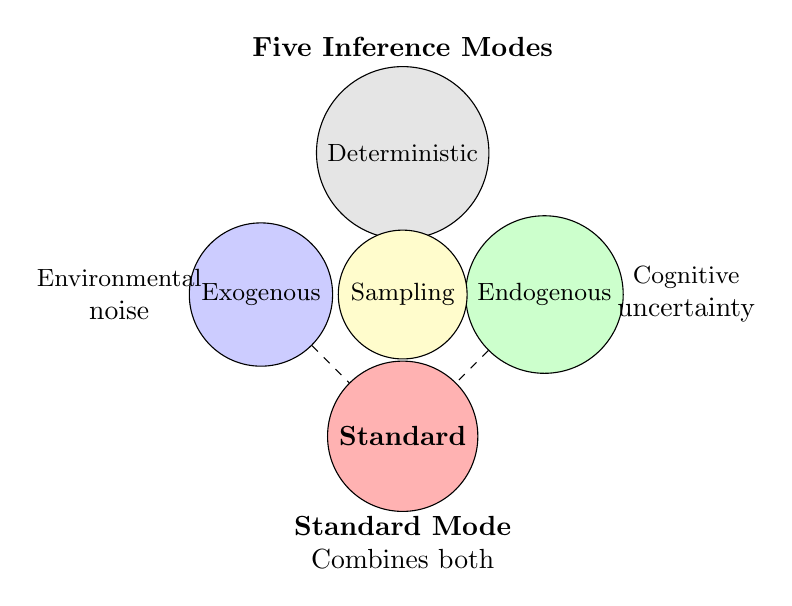
\begin{tikzpicture}[scale=0.9]
% 画五个圆圈代表五种模式
\node[circle, draw, fill=gray!20, minimum size=1.5cm] (det) at (0,2) {\small Deterministic};
\node[circle, draw, fill=blue!20, minimum size=1.5cm] (exo) at (-2,0) {\small Exogenous};
\node[circle, draw, fill=green!20, minimum size=1.5cm] (endo) at (2,0) {\small Endogenous};
\node[circle, draw, fill=red!30, minimum size=1.8cm] (std) at (0,-2) {\textbf{Standard}};
\node[circle, draw, fill=yellow!20, minimum size=1.5cm] (samp) at (0,0) {\small Sampling};

% 连线
\draw[dashed] (exo) -- (std);
\draw[dashed] (endo) -- (std);

% 说明
\node at (0,3.5) {\textbf{Five Inference Modes}};
\node[align=center] at (-4,0) {\small Environmental\\noise};
\node[align=center] at (4,0) {\small Cognitive\\uncertainty};
\node[align=center] at (0,-3.5) {\textbf{Standard Mode}\\Combines both};
\end{tikzpicture}
\end{center}

\begin{alertblock}{推荐使用 (Recommended)}
\textbf{标准模式 (Standard mode)} 在大多数实际应用中效果最好! (works best in most real applications!)
\end{alertblock}
\end{frame}

% 第四部分:性能有多好?
\section{因果引擎的性能有多好? (How good is the performance?)}

\begin{frame}{抗噪音能力测试: 回归任务 (Noise Robustness Test: Regression)}
\begin{columns}
\column{0.5\textwidth}
\begin{center}
\textbf{随着噪音增加, 性能如何变化? (How does performance change with noise?)}
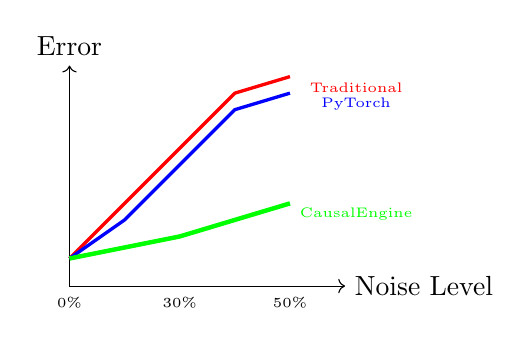
\begin{tikzpicture}[scale=0.7]
\draw[->] (0,0) -- (5,0) node[right] {Noise Level};
\draw[->] (0,0) -- (0,4) node[above] {Error};

% 性能曲线(简化)
\draw[red, very thick] (0,0.5) -- (1,1.5) -- (2,2.5) -- (3,3.5) -- (4,3.8);
\draw[blue, very thick] (0,0.5) -- (1,1.2) -- (2,2.2) -- (3,3.2) -- (4,3.5);
\draw[green, ultra thick] (0,0.5) -- (1,0.7) -- (2,0.9) -- (3,1.2) -- (4,1.5);

% 图例
\node[red] at (5.2,3.6) {\tiny Traditional};
\node[blue] at (5.2,3.3) {\tiny PyTorch};
\node[green] at (5.2,1.3) {\tiny CausalEngine};

% X轴标签
\node at (0,-0.3) {\tiny 0\%};
\node at (2,-0.3) {\tiny 30\%};
\node at (4,-0.3) {\tiny 50\%};
\end{tikzpicture}
\end{center}

\column{0.5\textwidth}
\textbf{30\%标签噪音下的表现: (Performance at 30\% label noise:)}
\begin{itemize}
    \item Traditional MLP: Error 47.60
    \item PyTorch: Error 45.32
    \item \textcolor{green}{\textbf{CausalEngine: Error 11.41}}
\end{itemize}

\vspace{1em}
\begin{alertblock}{惊人提升 (Amazing improvement)}
\textbf{性能提升76\%! (76\% improvement!)}
\end{alertblock}
\end{columns}

\vspace{1em}
\begin{block}{关键发现 (Key Finding)}
噪音越多, 因果引擎的优势越明显! (More noise = more advantage for CausalEngine!)
\end{block}
\end{frame}

% 第五部分:怎么使用?
\section{怎么使用因果引擎? (How to use CausalEngine?)}

\begin{frame}[fragile]{安装和基本使用 (Installation and Basic Usage)}
\begin{block}{安装很简单 (Installation is simple)}
\begin{lstlisting}
pip install causal-sklearn
\end{lstlisting}
\end{block}

\begin{block}{基本使用示例 (Basic Usage Example)}
\begin{lstlisting}
from causal_sklearn import MLPCausalRegressor
from sklearn.datasets import make_regression
from sklearn.model_selection import train_test_split

# Generate data
X, y = make_regression(n_samples=1000, n_features=10, noise=20)
X_train, X_test, y_train, y_test = train_test_split(X, y)

# Create and train model
model = MLPCausalRegressor(
    hidden_layer_sizes=(100, 50),
    inference_mode='standard',  # Recommended mode
    max_iter=200
)
model.fit(X_train, y_train)

# Predict and evaluate
score = model.score(X_test, y_test)
print(f"Test score: {score:.4f}")
\end{lstlisting}
\end{block}
\end{frame}

% 第六部分:应用场景
\section{适用场景 (Use Cases)}

\begin{frame}{什么时候用因果引擎? (When to use CausalEngine?)}
\begin{columns}
\column{0.5\textwidth}
\textbf{特别适合的场景: (Particularly suitable:)}
\begin{itemize}
    \item $\checkmark$ 数据有很多噪音的时候 (Noisy data)
    \item $\checkmark$ 需要理解个体差异 (Individual differences matter)
    \item $\checkmark$ 医疗诊断 (Medical diagnosis)
    \item $\checkmark$ 金融风险评估 (Financial risk)
    \item $\checkmark$ 推荐系统 (Recommendation systems)
    \item $\checkmark$ 异常检测 (Anomaly detection)
\end{itemize}

\column{0.5\textwidth}
\textbf{优势不明显的场景: (Limited advantage:)}
\begin{itemize}
    \item $\times$ 数据非常干净 (Very clean data)
    \item $\times$ 纯图像分类 (Pure image classification)
    \item $\times$ 不需要解释性的场景 (No interpretability needed)
    \item $\times$ 计算资源极其有限 (Very limited computation)
\end{itemize}
\end{columns}

\vspace{1em}
\begin{block}{经验法则 (Rule of thumb)}
当数据质量不确定或需要鲁棒性时, 因果引擎是理想选择 (When data quality is uncertain or robustness is needed, CausalEngine is ideal)
\end{block}
\end{frame}

% 第七部分:总结
\section{总结与展望 (Summary and Outlook)}

\begin{frame}{核心贡献 (Core Contributions)}
\begin{enumerate}
    \item \textbf{新的机器学习范式 (New ML Paradigm)}
    \begin{itemize}
        \item 从学习相关性到学习因果关系 (From correlation to causation)
        \item 把个体差异当作特征, 而不是噪音 (Individual differences as features, not noise)
    \end{itemize}
    
    \item \textbf{实用的实现 (Practical Implementation)}
    \begin{itemize}
        \item 完全兼容scikit-learn API (Full scikit-learn compatibility)
        \item 高效的分析计算 (Efficient analytical computation)
        \item 容易集成到现有工作流程 (Easy integration)
    \end{itemize}
    
    \item \textbf{出色的鲁棒性 (Exceptional Robustness)}
    \begin{itemize}
        \item 在噪音环境中性能优异 (Superior performance in noisy environments)
        \item 适合现实世界的混乱数据 (Suitable for real-world messy data)
    \end{itemize}
\end{enumerate}

\vspace{1em}
\begin{block}{一句话总结 (One-sentence Summary)}
因果引擎通过理解"为什么"而不仅仅是"是什么", 为机器学习带来新的可能性 (CausalEngine brings new possibilities to ML by understanding WHY, not just WHAT)
\end{block}
\end{frame}

\begin{frame}
\begin{center}
{\Huge \textbf{谢谢大家! (Thank You!)}}

\vspace{2em}

{\Large 有问题可以讨论 (Questions \& Discussion)}

\vspace{2em}

{\large 让机器学习变得更智能 (Making ML Smarter) 🚀}
\end{center}
\end{frame}

\end{document}